\documentclass[12pt,a4paper]{article}
\usepackage{graphicx,amsmath}
%\usepackage{subfigure}
\usepackage{float}
\usepackage[german]{babel}
\usepackage[utf8]{inputenc}
\setcounter{secnumdepth}{4}
\usepackage[top=2cm, bottom=2.5cm, left=3cm, right=3cm]{geometry}
\begin{document}


%\title{Bachelorarbeit}
%\author{Richard Kullmann}
%\date{02.06.2017}

\thispagestyle{empty}
%\setcounter{page}{2}
\newpage
\tableofcontents
\thispagestyle{empty}
\newpage
\pagenumbering{arabic}

\section{Gleichgewichtspunkte und Stabilität}
Um verschiedene Modelle zu vergleichen, kann es hilfreich sein, eine Phasenraumanalyse durchzuführen. Diese beinhaltet das Ermitteln der Isoklinen sowie die Überprüfung der sich daraus ergebenden Gleichgewichtspunkte auf ihre Stabilität. 
\subsection{$I_{Na,p}+I_K$-Modell}
Als erstes bietet es sich an, die Isoklinen darzustellen, die sich bei den dynamischen Variablen $V$ und $n$ aus $\dot{V}=0$ und $\dot{n}=0$ ergeben. Somit ergibt sich für die V-Isokline:
\begin{align*} 
n=\frac{I-g_L(V-E_L)-G_{Na}m_{\infty}(V)(V-E_{Na})}{g_K(V-E_K)}
\end{align*}
Sowie für die n-Isokline:
\begin{align}
n=n_{\infty}(V)=\frac{1}{1+\exp\left(\frac{V_{1/2}-V}{k}\right)}
\end{align}
Daraus erhält man folgendes Bild des Phasenraums: 
\begin{figure}[H]
	\centering
	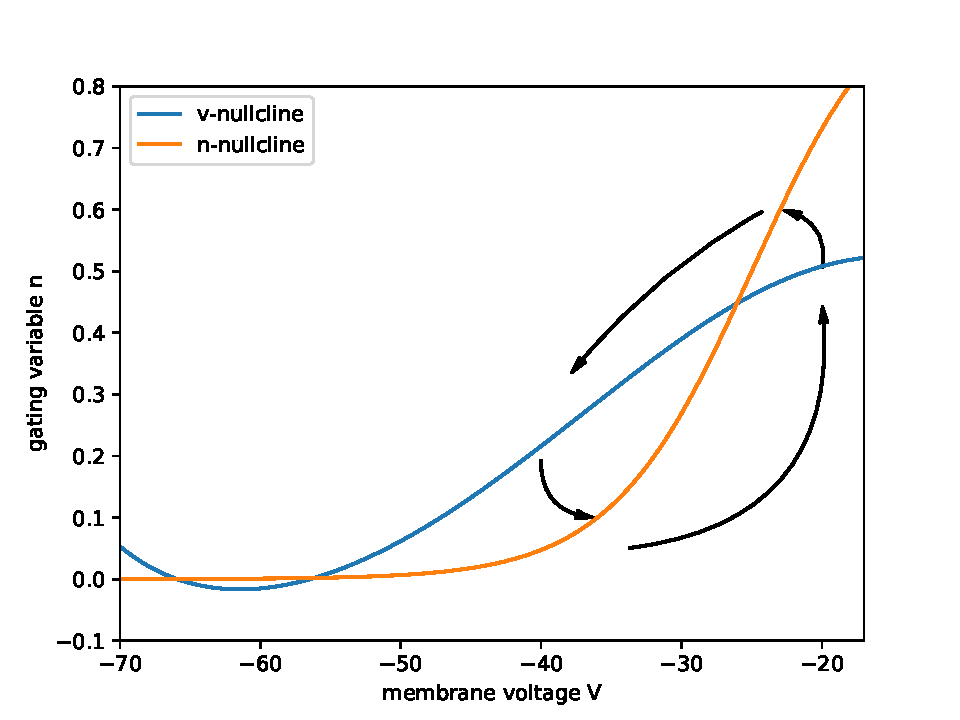
\includegraphics[scale=0.9]{inapiknc1.pdf} 
	\caption{Isoklinen im $I_{Na,p}+I_K$-Modell mit I=0. Die Pfeile geben die Richtung des Vektorfelds in den verschiedenen Bereichen an, in die die Isoklinen den Phasenraum aufteilen}
	\label{niso}
\end{figure} 
Es sind 3 Schnittpunkte der Isoklinen zu erkennen, bei etwa -66,-56 und -26 mV. Jeder dieser Schnittpunkte entspricht einem Gleichgewichtspunkt des Systems. 
\subsubsection{Lokale lineare Analyse}
Die Stabilität der gefunden Gleichgewichtspunkte kann mittels der lokalen linearen Analyse gefunden werden. Für ein allgemeines zweidimensionales Modell der Form
\begin{align}
\dot{x}=f(x,y)\\
\dot{y}=g(x,y)
\end{align}
macht man sich dabei die Möglichkeit zunutze, dass die Funktionen $f$ und $g$ im Gleichgewicht durch Geraden angenähert werden können, also mit der ersten Ordnung der entsprechenden Taylorreihen-Entwicklung. Nahe des Gleichgewichtspunkts ($x_0$,$y_0$) findet man dann ein lineares System:
\begin{align}				
\left(\begin{matrix}\dot{u}\\\dot{w}
\end{matrix}\right)
=\left(\begin{matrix}a b\\
c d\end{matrix}\right)\left(\begin{matrix}u\\w\end{matrix}\right)=L\left(\begin{matrix}u\\w\end{matrix}\right)
\end{align}
mit den partiellen Ableitungen
\begin{align}
a=\frac{\partial f}{\partial x}(x_0,y_0),\qquad b=\frac{\partial f}{\partial y}(x_0,y_0) \\
c=\frac{\partial g}{\partial x}(x_0,y_0),\qquad d=\frac{\partial g}{\partial y}(x_0,y_0)
\end{align}
sowie $u=x-x_0$ und $w=y-y_0$. $L$ ist die Jacobi-Matrix des Systems im Gleichgewicht. Die Eigenwerte dieser Matrix
\begin{align}
\lambda_{1,2}=\frac{\tau\pm\sqrt{\tau^2-4\Delta}}{2}\qquad \text{mit}\quad \tau=a+d, \Delta=ad-bc
\end{align} bestimmen über das Verhalten des Systems im Gleichgewicht und dementsprechend über die Stabilität des Gleichgewichtspunkts. Haben beide Eigenwerte einen positiven Realteil, ist der Gleichgewichtspunkt instabil, bei negativem Realteil ist er stabil. Bei nichtverschwindendem Imaginärteil liegt ein Fokus vor, um den die Trajektorien rotieren. Haben die reellen Eigenwerte entgegengesetzte Vorzeichen, handelt es sich um einen Sattel. Dieser ist ebenfalls instabil, allerdings nähern sich die meisten Trajektorien zunächst an einen derartigen Punkt an, bevor sie divergieren.
\\\\
Wendet man diese Methode auf obiges Modell an, erhält man folgende Werte:
\begin{align*}
\lambda_1(-66)&=-1.74876 & \lambda_2(-66)&=-6.5626\\
\lambda_1(-56)&=1.9425& \lambda_2(-56)&=-6.48719\\
\lambda_1(-26)&=0.464453 + 11.7323i& \lambda_2(-26)&=0.464453 - 11.7323i
\end{align*}
Der linke Gleichgewichtspunkt ist also ein stabiler Knoten, der mittlere ein Sattelpunkt und der rechte ein instabiler Fokus. Um dementsprechend bei schnellem $K^+$-Strom vom Grenzzyklus zum stabilen Punkt zu gelangen, reicht eine geringe Störung, da der Grenzzyklus den Sattelpunkt passiert, um allerdings vom stabilen Punkt wieder den burstenden Zustand zu erreichen, ist eine stärkere Störung notwendig.
\subsection{Mechanisches Modell}
Die gleichen Betrachtungen können auch für das mechanische Modell durchgeführt werden. Dort wurden Brownsche Teilchen in einem gekippten Cosinus-Potenzial simuliert:
\begin{align*}
\dot{x}&=v\\
\dot{v}&=-\gamma v-U'(x)+\sqrt{2\gamma kT}\xi(t)
\end{align*}
mit $U(x)=-Fx-d\cos(x)$ sowie $\gamma=0.4$ und $d=1$. Die $x$-Isokline ist 0, und die $v$-Isokline ist ein simpler Sinus:
\begin{figure}[H]
	\centering
	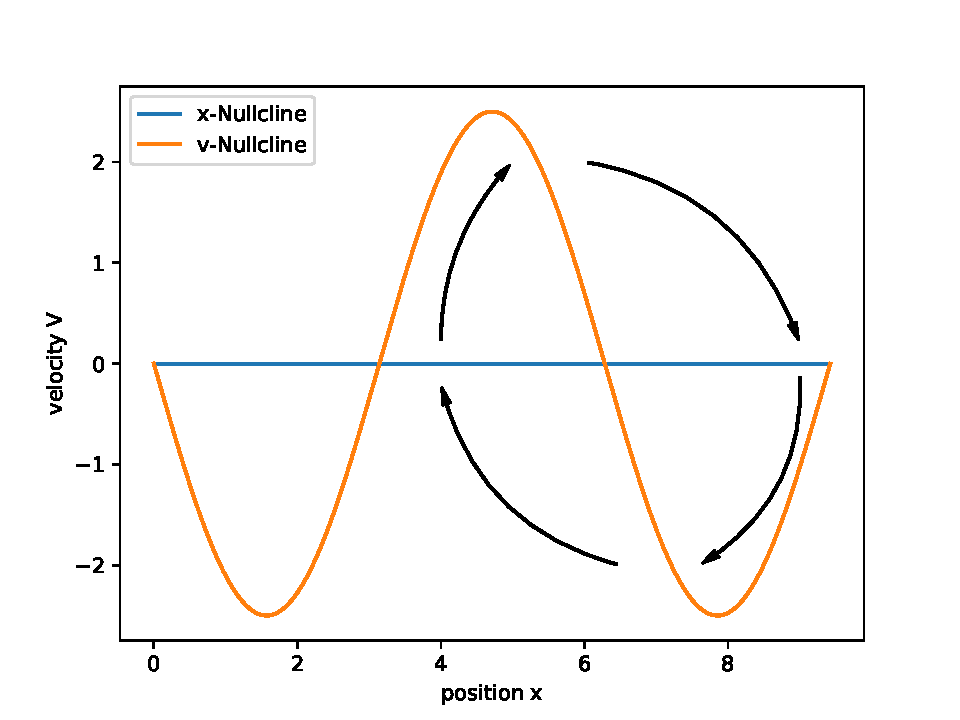
\includegraphics[scale=0.9]{nullclinemm.pdf} 
	\caption{Isoklinen eines Brownschen Teilchens im Cosinunspotential bei F=0}
	\label{miso}
\end{figure} 
Die Gleichgewichtspunkte erfüllen die Gleichung
\begin{align}
\sin(x)=\frac{F}{d}
\end{align}
Für $F=0$ wird diese durch Vielfache von $\pi$ gelöst. Aufgrund der Periodizität der Isoklinen genügt es, zwei aufeinanderfolgende Gleichgewichtspunkte zu untersuchen. Aus $\tau=\gamma$ und $\Delta=d\cos(x)$ folgt dann für die Eigenwerte:
\begin{align*}
\lambda_{1,2}(x=0)&=-0.4\pm\sqrt{-3.84}\\\lambda_{1,2}(x=\pi)&=-0.4\pm\sqrt{4.16}
\end{align*}
Bei $x=n\pi$ befindet sich also ein stabiler Fokus, bei $x=(n+1)\pi$ liegt ein instabiler Knoten vor.\\
Dies wirft noch einmal ein anderes Licht auf das Phasenraumporträt des mechanischen Modells. Der scheinbar existierende Grenzzyklus stellt tatsächlich nur das oszillierende Annähern an den stabilen Fokus dar, produziert also keine Spikes.\\
Für die Darstellung des burstenden Zustands innerhalb einer Periode eignet sich daher das folgende Phasenporträt besser:
\begin{figure}[H]
	\centering
	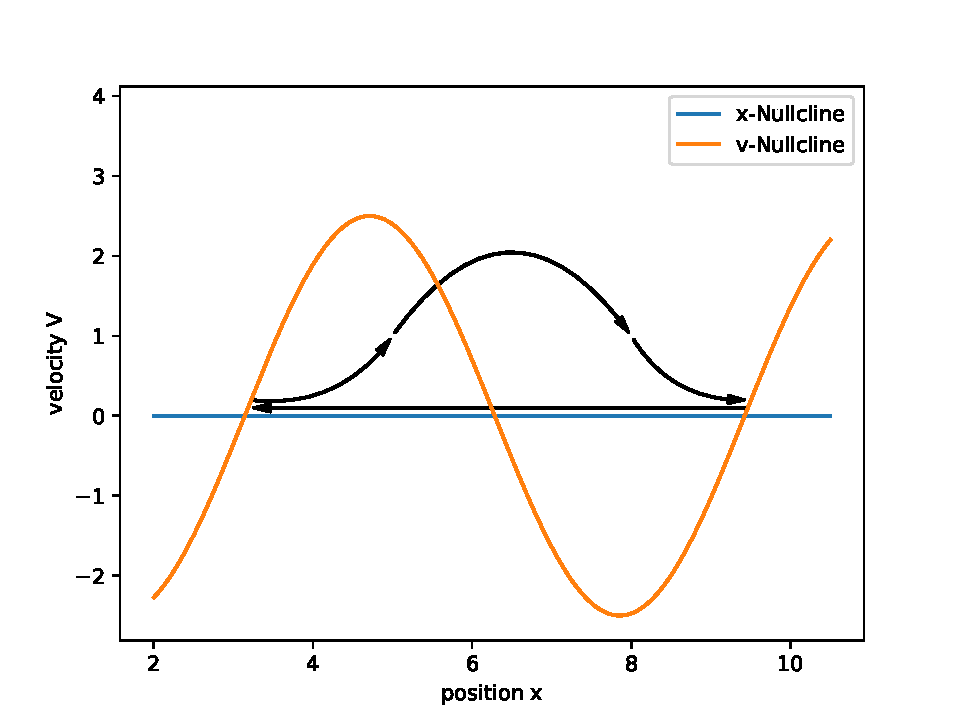
\includegraphics[scale=0.9]{nullclinemm3.pdf} 
	\caption{Stabiler Grenzzyklus eines Brownschen Teilchens im Cosinunspotential bei F=0}
	\label{miso2}
\end{figure} 
Nachdem das Teilchen eine Periode durchlaufen hat, findet es die selben Bedingungen wie am Anfang der Periode vor; ein simples Zurücksetzen an die entsprechende um $2\pi$ verschobene Stelle ändert also nichts am Verhalten.\\
Versucht man dieses Phasenporträt auch in einem Neuronenmodell zu finden, muss man also nach einem Modell mit einem instabilen Knoten und einem stabilen Fokus suchen. Das ist tatsächlich durchaus mit leichten Anpassungen des $I_{Na,p}+I_K$-Modells möglich, wenn man in Kauf nimmt, dass es dann noch einen dritten Gleichgewichtspunkt gibt. Zusätzlich ist es auch nicht so einfach, den stabilen Fokus bis zu einem Bias-Strom aufrechtzuerhalten, an dem $D_{eff}$ sein Maximum erreicht. Viel schwieriger ist allerdings die qualitative Reproduktion des Grenzzyklus. Die Position $x$ im mechanischen Modell ist mit der Spannung $V$ im Neuronenmodell zu identifizieren, die Geschwindigkeit mit der Gating-Variablen. Unabhängig davon, an welcher Stelle man den rückwärtigen Pfeil ansetzt (man kann das natürlich an einem beliebigen Punkt tun), weist der Grenzzyklus stets eine Unstetigkeit auf. Und eine derartige Unstetigkeit tritt so nicht in einem Neuronenmodell auf und lässt sich demnach nicht so einfach realisieren. \\
Diese beiden Beobachtungen liefern jedenfalls eine Erklärung, warum das bisher verwendete Modell nicht das erwartete Verhalten zeigt. Die Frage bleibt nun allerdings, ob oben genannte Bedingungen zulänglich von einem existierenden Neuronenmodell erfüllt werden, mit dem dann neue Simulationen gestartet werden können.
\end{document}